%% abtex2-modelo-trabalho-academico.tex, v-1.9.3 laurocesar
%% Copyright 2012-2015 by abnTeX2 group at http://abntex2.googlecode.com/ 
%% This work may be distributed and/or modified under the
%% conditions of the LaTeX Project Public License, either version 1.3
%% of this license or (at your option) any later version.
%% The latest version of this license is in
%%   http://www.latex-project.org/lppl.txt
%% and version 1.3 or later is part of all distributions of LaTeX
%% version 2005/12/01 or later.
%%
%% This work has the LPPL maintenance status `maintained'.
%% 
%% The Current Maintainer of this work is the abnTeX2 team, led
%% by Lauro César Araujo. Further information are available on 
%% http://abntex2.googlecode.com/
%%
%% This work consists of the files abntex2-modelo-trabalho-academico.tex,
%% abntex2-modelo-include-comandos and abntex2-modelo-references.bib
%%

% ------------------------------------------------------------------------
% ------------------------------------------------------------------------
% abnTeX2: Modelo de Trabalho Academico (tese de doutorado, dissertacao de
% mestrado e trabalhos monograficos em geral) em conformidade com 
% ABNT NBR 14724:2011: Informacao e documentacao - Trabalhos academicos -
% Apresentacao
% ------------------------------------------------------------------------
% ------------------------------------------------------------------------

\documentclass[
	% -- opções da classe memoir --
	12pt,				% tamanho da fonte
	openright,			% capítulos começam em pág ímpar (insere página vazia caso preciso)
	twoside,			% para impressão em verso e anverso. Oposto a oneside
	a4paper,			% tamanho do papel. 
	% -- opções da classe abntex2 --
	%chapter=TITLE,		% títulos de capítulos convertidos em letras maiúsculas
	%section=TITLE,		% títulos de seções convertidos em letras maiúsculas
	%subsection=TITLE,	% títulos de subseções convertidos em letras maiúsculas
	%subsubsection=TITLE,% títulos de subsubseções convertidos em letras maiúsculas
	% -- opções do pacote babel --
	english,			% idioma adicional para hifenização
	brazil				% o último idioma é o principal do documento
	]{abntex2}

% ---
% Pacotes básicos 
% ---
\usepackage{uarial}				% Usa a fonte Latin Modern			lmodern
\usepackage[T1]{fontenc}		% Selecao de codigos de fonte.
\usepackage[utf8]{inputenc}		% Codificacao do documento (conversão automática dos acentos)
\usepackage{lastpage}			% Usado pela Ficha catalográfica
\usepackage{indentfirst}		% Indenta o primeiro parágrafo de cada seção.
\usepackage{color}				% Controle das cores
\usepackage{graphicx}			% Inclusão de gráficos
\usepackage{microtype} 			% para melhorias de justificação

% pacotes adicionados
\usepackage{amsmath}
\usepackage{amssymb,amsfonts,amsthm}
\usepackage{setspace}
% ---
		
% ---
% Pacotes adicionais, usados apenas no âmbito do Modelo Canônico do abnteX2
% ---
\usepackage{lipsum}				% para geração de dummy text
% ---
\usepackage{todonotes}
% ---
% Pacotes de citações
% ---
\usepackage[brazilian,hyperpageref]{backref}	 % Paginas com as citações na bibl
\usepackage[alf]{abntex2cite}	% Citações padrão ABNT


\renewcommand{\bf}[1]{\mathbf{#1}}
\renewcommand{\rm}[1]{\mathrm{#1}}


\usepackage{cite}
\renewcommand\citeleft{[}
\renewcommand\citeright{]}

% --- 
% CONFIGURAÇÕES DE PACOTES
% --- 
\renewcommand{\imprimircapa}{
\thispagestyle{empty}

\vfill
 \begin{center}
    

    {\large\bfseries UNIVERSIDADE ESTADUAL DE SANTA CRUZ} \\
    
   
    {\large\bfseries CAMPUS Prof. SOANE NAZARÉ DE ANDRADE}  \\ 

    \vspace*{1in}
    \begin{large} \bfseries NOME DO ALUNO \end{large}\\[0.4in]

    \vspace*{4cm}
    \noindent \\
    
    \large\bfseries{TÍTULO DO TRABALHO} \\
    \vfill
    \large\bfseries{ ILHÉUS \\ 2017}
\end{center}

\normalsize


}


\renewcommand{\imprimirfolhaderosto}{

\begin{center}

    {\large NOME DO ALUNO\\}
    \vspace{8cm}
    {\Large \textsc\textbf{{TÍTULO DO TRABALHO} }\\}
    \vspace{1cm}
    \hspace{.45\linewidth}
    \begin{minipage}{.50\linewidth}

            \textbf{Trabalho de Conclusão de Curso submetido à Universidade Estadual de Santa Cruz,  como requisito 
            necessário para obtenção do grau de Bacharel em Ciência de Computação }

           
    
    \end{minipage}

    \vspace{2cm}
    \vfill
    {\large Ilhéus, janeiro de 2017}
\end{center}

}


% ---
% Configurações do pacote backref
% Usado sem a opção hyperpageref de backref
\renewcommand{\backrefpagesname}{Citado na(s) página(s):~}
% Texto padrão antes do número das páginas
\renewcommand{\backref}{}
% Define os textos da citação
\renewcommand*{\backrefalt}[4]{
	\ifcase #1 %
		Nenhuma citação no texto.%
	\or
		Citado na página #2.%
	\else
		Citado #1 vezes nas páginas #2.%
	\fi}%
% ---
% ---
% Informações de dados para CAPA e FOLHA DE ROSTO
% ---

\titulo{Título do Trabalho}
\autor{Aluno}
\local{Brasil}
\data{2017, v-1.9.3}
\orientador{Orientador}
\coorientador{coorientador}
\instituicao{%
  Universidade Estadual de Santa Cruz
  \par
  Departamento de Ciências Exatas e Tecnológicas
  }
\tipotrabalho{Projeto de Fim de Curso}
% O preambulo deve conter o tipo do trabalho, o objetivo, 
% o nome da instituição e a área de concentração 
\preambulo{O preambulo deve conter o tipo do trabalho, o objetivo, o nome da instituição e a área de concentração }
% ---






% ---
% Configurações de aparência do PDF final

% alterando o aspecto da cor azul
\definecolor{blue}{RGB}{41,5,195}

% informações do PDF
\makeatletter
\hypersetup{
     	%pagebackref=true,
		colorlinks=true,       		% false: boxed links; true: colored links
    	linkcolor=blue,          	% color of internal links
    	citecolor=black,        		% color of links to bibliography
    	filecolor=magenta,      		% color of file links
		urlcolor=blue,
		bookmarksdepth=4
}



\makeatother
% --- 

% --- 
% Espaçamentos entre linhas e parágrafos 
% --- 

% O tamanho do parágrafo é dado por:
\setlength{\parindent}{1.3cm}

% Controle do espaçamento entre um parágrafo e outro:
\setlength{\parskip}{0.2cm}  % tente também \onelineskip

% ---
% compila o indice
% ---
\makeindex
% ---

% ----
% Início do documento
% ----
\begin{document}

% Seleciona o idioma do documento (conforme pacotes do babel)
%\selectlanguage{english}
\selectlanguage{brazil}

% Retira espaço extra obsoleto entre as frases.
\frenchspacing 

% ----------------------------------------------------------
% ELEMENTOS PRÉ-TEXTUAIS
% ----------------------------------------------------------
\pretextual

% ---
% Capa
% ---
\imprimircapa
% ---

% ---
% Folha de rosto
% (o * indica que haverá a ficha bibliográfica)
% ---
\imprimirfolhaderosto

% ---
% Inserir a ficha bibliografica
% ---

% Isto é um exemplo de Ficha Catalográfica, ou ``Dados internacionais de
% catalogação-na-publicação''. Você pode utilizar este modelo como referência. 
% Porém, provavelmente a biblioteca da sua universidade lhe fornecerá um PDF
% com a ficha catalográfica definitiva após a defesa do trabalho. Quando estiver
% com o documento, salve-o como PDF no diretório do seu projeto e substitua todo
% o conteúdo de implementação deste arquivo pelo comando abaixo:
%
% \begin{fichacatalografica}
%     \includepdf{fig_ficha_catalografica.pdf}
% \end{fichacatalografica}

\begin{fichacatalografica}
%	\sffamily
%	\vspace*{\fill}					% Posição vertical
%	\begin{center}					% Minipage Centralizado
%	\fbox{\begin{minipage}[c][8cm]{13.5cm}		% Largura
%	\small
%	\imprimirautor
%	%Sobrenome, Nome do autor
%	
%	\hspace{0.5cm} \imprimirtitulo  / \imprimirautor. --
%	\imprimirlocal, \imprimirdata-
%	
%	\hspace{0.5cm} \pageref{LastPage} p. : il. (algumas color.) ; 30 cm.\\
%	
%	\hspace{0.5cm} \imprimirorientadorRotulo~\imprimirorientador\\
%	
%	\hspace{0.5cm}
%	\parbox[t]{\textwidth}{\imprimirtipotrabalho~--~\imprimirinstituicao,
%	\imprimirdata.}\\
%	
%	\hspace{0.5cm}
%		1. Palavra-chave1.
%		2. Palavra-chave2.
%		2. Palavra-chave3.
%		I. Orientador.
%		II. Universidade xxx.
%		III. Faculdade de xxx.
%		IV. Título 			
%	\end{minipage}}
%	\end{center}
\end{fichacatalografica}
%% ---
% Inserir errata
% ---
\begin{errata}
Elemento opcional da \citeonline[4.2.1.2]{NBR14724:2011}. Exemplo:

\vspace{\onelineskip}

FERRIGNO, C. R. A. \textbf{Tratamento de neoplasias ósseas apendiculares com
reimplantação de enxerto ósseo autólogo autoclavado associado ao plasma
rico em plaquetas}: estudo crítico na cirurgia de preservação de membro em
cães. 2011. 128 f. Tese (Livre-Docência) - Faculdade de Medicina Veterinária e
Zootecnia, Universidade de São Paulo, São Paulo, 2011.

\begin{table}[htb]
\center
\footnotesize
\begin{tabular}{|p{1.4cm}|p{1cm}|p{3cm}|p{3cm}|}
  \hline
   \textbf{Folha} & \textbf{Linha}  & \textbf{Onde se lê}  & \textbf{Leia-se}  \\
    \hline
    1 & 10 & auto-conclavo & autoconclavo\\
   \hline
\end{tabular}
\end{table}

\end{errata}
% ---

% ---
% Inserir folha de aprovação
% ---

% Isto é um exemplo de Folha de aprovação, elemento obrigatório da NBR
% 14724/2011 (seção 4.2.1.3). Você pode utilizar este modelo até a aprovação
% do trabalho. Após isso, substitua todo o conteúdo deste arquivo por uma
% imagem da página assinada pela banca com o comando abaixo:
%
% \includepdf{folhadeaprovacao_final.pdf}
%
\begin{folhadeaprovacao}


\begin{center}


            {UNIVERSIDADE ESTADUAL DE SANTA CRUZ} \\
           

    \vspace{1.5cm}
                                    {NOME DO ALUNO}\\
    \bfseries{}
\end{center}

Esta Monografia foi julgada adequada para a obten\c{c}\~{a}o do título  de Bacharel em Ciência de Computação, sendo aprovada em sua forma final  pela banca examinadora:

    \vspace{2.5cm}
    \assinatura{Orientador(a): Prof. Dr. XXXXXXX \\ Universidade XXXXXXX}
    \assinatura{Prof. Dr. xxxxxxx \\ Universidade ccccccccc}
    \assinatura{Prof. Dr. ononononononon \\ Universidade ononononononon}
    \vspace{3 cm}%\vfill

    \begin{center}
        Ilhéus, XX de janeiro de 2017
    \end{center}
  
\end{folhadeaprovacao}
%% ---
% Dedicatória
% ---
\begin{dedicatoria}
   \vspace*{\fill}
   \centering
   \noindent
   \textit{ Este trabalho é dedicado às crianças adultas que,\\
   quando pequenas, sonharam em se tornar cientistas.} \vspace*{\fill}
\end{dedicatoria}
% ---
% ---
% Agradecimentos
% ---
\begin{agradecimentos}
ou Acknowledgements, se em inglês \\
Opcional

\end{agradecimentos}
% ---
%% ---
% Epígrafe
% ---
\begin{epigrafe}
    \vspace*{\fill}
	\begin{flushright}
		\textit{``Não vos amoldeis às estruturas deste mundo, \\
		mas transformai-vos pela renovação da mente, \\
		a fim de distinguir qual é a vontade de Deus: \\
		o que é bom, o que Lhe é agradável, o que é perfeito.\\
		(Bíblia Sagrada, Romanos 12, 2)}
	\end{flushright}
\end{epigrafe}
% ---

% ---
% RESUMOS
% ---

% resumo em português
\setlength{\absparsep}{18pt} % ajusta o espaçamento dos parágrafos do resumo
\begin{resumo}
Coloque aqui o resumo de seu trabalho.


 \textbf{Palavras-chave}:.
\end{resumo}

% resumo em inglês
\begin{resumo}[Abstract]
 \begin{otherlanguage*}{english}
Resumo em Inglês
   \vspace{\onelineskip}
 
   \noindent 
   \textbf{Keywords}:Palavras Chaves.
 \end{otherlanguage*}
\end{resumo}

%% resumo em francês 
%\begin{resumo}[Résumé]
% \begin{otherlanguage*}{french}
%    Il s'agit d'un résumé en français.
% 
%   \textbf{Mots-clés}: latex. abntex. publication de textes.
% \end{otherlanguage*}
%\end{resumo}
%
%% resumo em espanhol
%\begin{resumo}[Resumen]
% \begin{otherlanguage*}{spanish}
%   Este es el resumen en español.
%  
%   \textbf{Palabras clave}: latex. abntex. publicación de textos.
% \end{otherlanguage*}
%\end{resumo}
% ---

% ---
% inserir lista de ilustrações
% ---
\pdfbookmark[0]{\listfigurename}{lof}
\listoffigures*
\cleardoublepage
%% ---

% ---
% inserir lista de tabelas
% ---
\pdfbookmark[0]{\listtablename}{lot}
\listoftables*
\cleardoublepage
% ---
% ---
% inserir lista de abreviaturas e siglas
% ---
\begin{siglas}
 \item Lista de Siglas
\end{siglas}
% ---

% ---
% inserir lista de símbolos
% ---
%\begin{simbolos}
%  \item[$ CO_2 $] Dióxido de Carbono
%  \item[$C_{3+}$] Hidrocarbonetos com três ou mais carbonos
%\end{simbolos}
% ---





% ---
% inserir o sumario
%% ---
\pdfbookmark[0]{\contentsname}{toc}
\tableofcontents*
\cleardoublepage
%% ---



% ----------------------------------------------------------
% ELEMENTOS TEXTUAIS
% ----------------------------------------------------------
\textual

\chapter{Introdução}

\section{Justificativa}

\section{Objetivo}

\subsection{ Objetivo Geral}

\subsection{Objetivos Específicos}


\section{Organização}
O presente trabalho está organizado da seguinte forma:





% Introduzir Figura
%\begin{figure}
%	   \centering
%	   		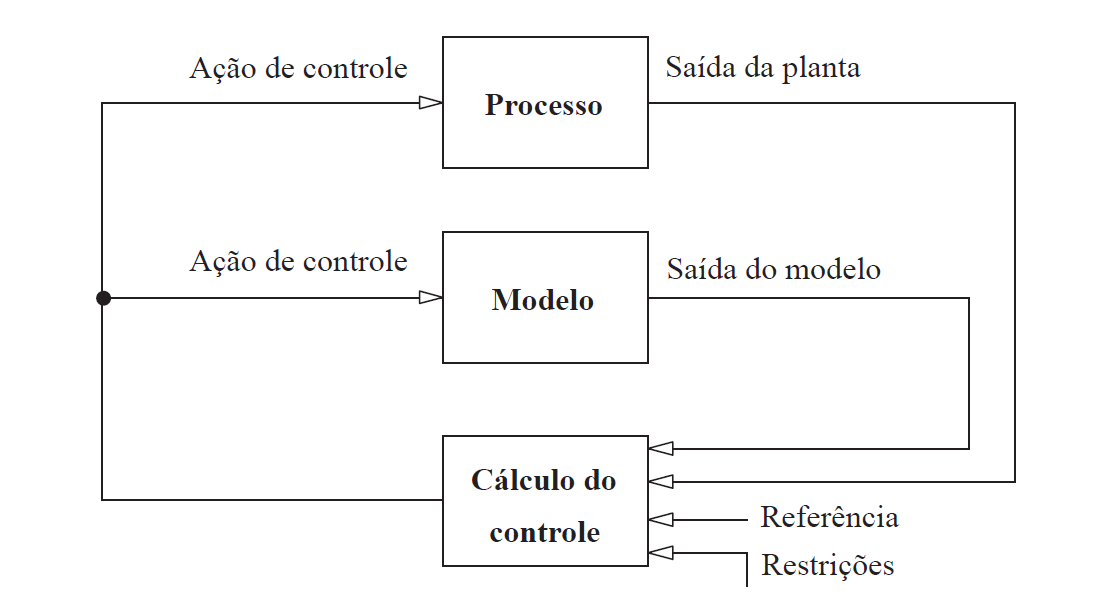
\includegraphics[scale=0.35]{figs/MPCbase.PNG} 
%	   \caption{Algoritmo MPC}
%	   \label{label para referencia cruzada Figura}
%\end{figure}


% Lista de Item

%\begin{itemize}
%	\item item 1
%	\item item 2
%	\item item 3
%\end{itemize}

% Equação
%\begin{equation}
%	\label{label para referencia cruzada %equacoes} 
%	y(t)=\sum_{i=1}^{\infty}h_i\Delta u(t-i)
%\end{equation}

% Equação em linha 
%$\hat{y}(t+k\mid t)= \sum^\infty_{i=1} g_i %\Delta u(t+k-i\mid t)$

% Citação -  Criei o arquivo de bibliografia usando o jabref

%\cite{Camacho2007} 

% Referencia Cruzada de Figura
%\ref{label para referencia cruzada Figura}

% Referencia Cruzada de Equação
%\ref{label para referencia cruzada equacoes}


% Tabelas

%\begin{table}[h]
%\begin{center}
%     \caption{Índices 1 para casos factíveis}
%     \begin{tabular}{| l | l | l | l |}
%     \hline Índice & LP Petro & LP 2 & %Diferença\\ 
%     \hline $SES_y$& 60.5406 & 60.5492 & %-0.0087\\
%     \hline $SES_u$& 1166.1464 & 1166.1464 & 2.36*$10^{-9}$ \\
%     \hline
 
%    \end{tabular}
%\label{table:indices1}
%\end{center}
%\end{table}
\chapter{\textit{Trabalhos Relacionados ou Revisão Bibiográfica}}



\chapter{Seu Trabalho}

\section{Metodologia}


\section{xxxxx}
\section{xxxxx}
\section{xxxxx}



\chapter{Avaliação}

\section{Aquisição do conhecimento}
\section{Modelo}
\section{Testes}
\section{Exemplos}

\chapter{conclusões}

%\chapter{Conclusão}




% ----------------------------------------------------------
% Finaliza a parte no bookmark do PDF
% para que se inicie o bookmark na raiz
% e adiciona espaço de parte no Sumário
% ----------------------------------------------------------
\phantompart

% ---
% Conclusão
% ---
%\chapter{Conclusão}
% ---

% ----------------------------------------------------------
% ELEMENTOS PÓS-TEXTUAIS
% ----------------------------------------------------------
\postextual
% ----------------------------------------------------------

% ----------------------------------------------------------
% Referências bibliográficas
% ----------------------------------------------------------
\bibliography{TCC.bib}

% ----------------------------------------------------------
% Glossário
% ----------------------------------------------------------
%
% Consulte o manual da classe abntex2 para orientações sobre o glossário.
%
%\glossary

%% ----------------------------------------------------------
% Apêndices
% ----------------------------------------------------------

% ---
% Inicia os apêndices
% ---
\begin{apendicesenv}

% Imprime uma página indicando o início dos apêndices
\partapendices

% ----------------------------------------------------------
\chapter{Quisque libero justo}
% ----------------------------------------------------------

\lipsum[50]

% ----------------------------------------------------------
\chapter{Nullam elementum urna vel imperdiet sodales elit ipsum pharetra ligula
ac pretium ante justo a nulla curabitur tristique arcu eu metus}
% ----------------------------------------------------------
\lipsum[55-57]

\end{apendicesenv}
% ---

%% ----------------------------------------------------------
% Anexos
% ----------------------------------------------------------

% ---
% Inicia os anexos
% ---
\begin{anexosenv}

% Imprime uma página indicando o início dos anexos
\partanexos

% ---
\chapter{Morbi ultrices rutrum lorem.}
% ---
\lipsum[30]

% ---
\chapter{Cras non urna sed feugiat cum sociis natoque penatibus et magnis dis
parturient montes nascetur ridiculus mus}
% ---

\lipsum[31]

% ---
\chapter{Fusce facilisis lacinia dui}
% ---

\lipsum[32]

\end{anexosenv}

%---------------------------------------------------------------------
% INDICE REMISSIVO
%---------------------------------------------------------------------
\phantompart
\printindex
%---------------------------------------------------------------------

\end{document}
